% This LaTeX was auto-generated from MATLAB code.
% To make changes, update the MATLAB code and export to LaTeX again.

\documentclass{article}

\usepackage[utf8]{inputenc}
\usepackage[T1]{fontenc}
\usepackage{lmodern}
\usepackage{graphicx}
\usepackage{color}
\usepackage{hyperref}
\usepackage{amsmath}
\usepackage{amsfonts}
\usepackage{epstopdf}
\usepackage[table]{xcolor}
\usepackage{matlab}

\sloppy
\epstopdfsetup{outdir=./}
\graphicspath{ {./seminar_live_images/} }

\matlabhastoc

\begin{document}

\label{T_253E321E}
\matlabtitle{Seminarski zadatak}

\matlabtableofcontents{Sadržaj}
\label{H_05D0154C}
\matlabheading{Uvod}

\label{H_1455D54F}
\matlabheadingtwo{U zadatku je potrebno:}

\begin{enumerate}
\setlength{\itemsep}{-1ex}
   \item{\begin{flushleft} Načiniti simulacijski model \textbf{nelinearnog }sustava u Simulinku i simuliratu odziv. \end{flushleft}}
   \item{\begin{flushleft} Zatvoriti povratnu vezu po položaju tereta (uzeti u obzir koeficijent povratne veze) i simulirati ponašanje sustava za pomak tereta iznosa 1 rad u lijevu i desnu stranu od srednjeg položaja motora. Prikazati na slikama ponašanje u vremenu za slijedeće varijable: referencu i ostvareni kut zakreta tereta, kutnu brzinu tereta, struju prop. ventila, pomak klipa prop ventila, protoke kroz prop. ventil, te tlakove u komorama motora. Pojačanjem regulatora ostvariti prihvatljiv odziv sustava. \end{flushleft}}
\end{enumerate}

\label{H_E9C20726}
\vspace{1em}

\label{H_BCC5041B}
\matlabheadingtwo{Opis zadatka}

\label{H_8B0C821E}
\matlabheadingthree{Slika hidrauličke sheme}

\begin{par}
\begin{flushleft}
Na slici je prikazan rotacijski hidraulički sustav, koji se sastoji od hidrauličkog motora upravljanog proporcionalnim ventilom, pri čemu se upravlja kutem zakreta tereta.
\end{flushleft}
\end{par}

\begin{par}
\begin{flushleft}
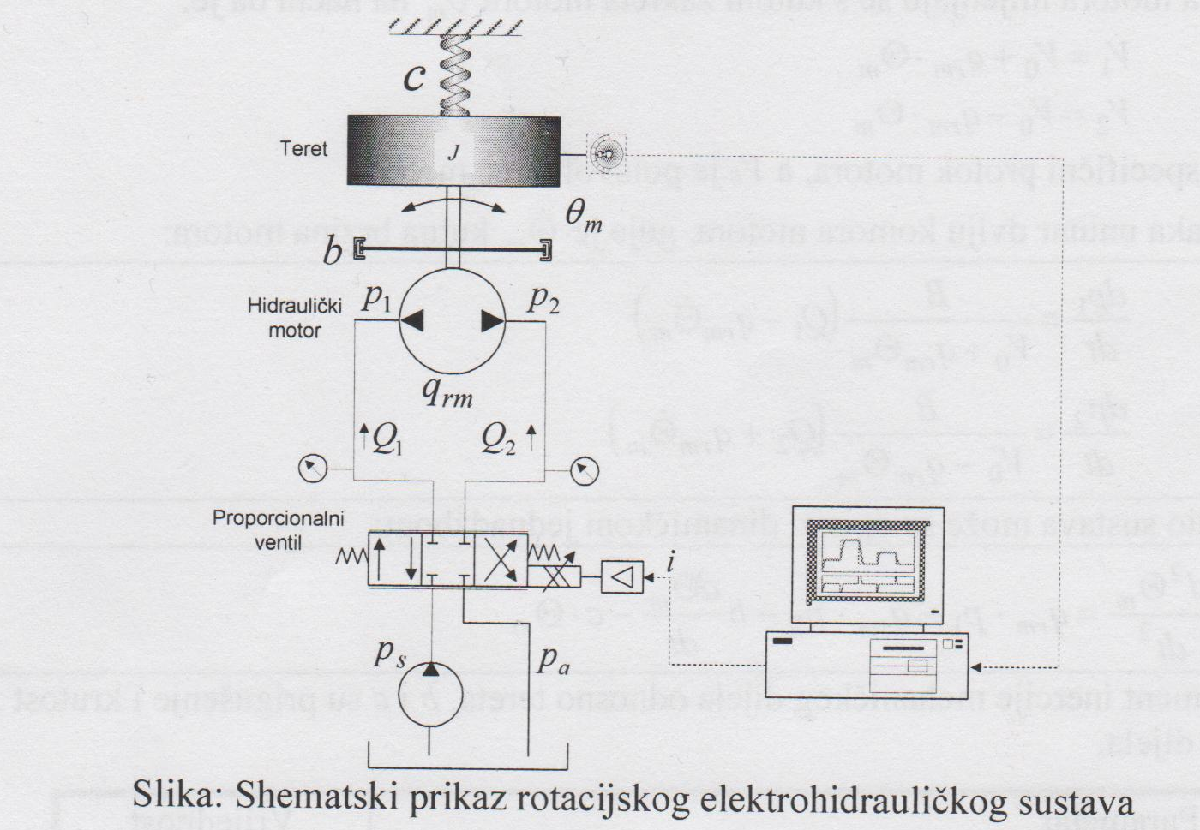
\includegraphics[width=\maxwidth{61.01354741595585em}]{image_0}
\end{flushleft}
\end{par}

\label{H_68A500C7}
\vspace{1em}


\vspace{1em}
\label{H_80365D62}
\matlabheadingthree{Proporcionalni ventil}

\label{H_7E0CEEEA}
\begin{par}
\begin{flushleft}
Dinamika proporcionalnog ventila može se opisati prijenosnom funkcijom P1 člana:
\end{flushleft}
\end{par}

\begin{par}
\begin{flushleft}
$\frac{y_v (s)}{i(s)}=\frac{K_v }{\frac{1}{\omega_v }+1}$        (1)
\end{flushleft}
\end{par}

\begin{par}
\begin{flushleft}
$y_v$ - pozicija klipa proporcionalnog ventila, m
\end{flushleft}
\end{par}

\begin{par}
\begin{flushleft}
$i$ - ulazna struja proporcionalnog ventila, A
\end{flushleft}
\end{par}

\begin{par}
\begin{flushleft}
$K_v$ - koeficijent pojačanja proporcionalnog ventila, m/A
\end{flushleft}
\end{par}

\begin{par}
\begin{flushleft}
$\omega_v$ - vlastita frekvencija proporcionalnog centila, rad/s
\end{flushleft}
\end{par}

\begin{par}
\begin{flushleft}
Jednadžbe protoka kroz proporcionalni ventil iznose:
\end{flushleft}
\end{par}

\begin{par}
\begin{flushleft}
$Q_1 (y_v ,p_1 )=\left\lbrace \begin{array}{cc}
y_v *\sqrt{|p_s -p_1 |}*sign(p_s -p_1 ), & \textrm{za}\;y_v \ge 0\\
y_v *\sqrt{|p_1 -p_s |}*sign(p_1 -p_s ), & \textrm{za}\;y_v <0
\end{array}\right.$        (2)
\end{flushleft}
\end{par}

\begin{par}
\begin{flushleft}
$Q_2 (y_v ,p_2 )=\left\lbrace \begin{array}{cc}
y_v *\sqrt{|p_2 -p_a |}*sign(p_2 -p_a ), & \textrm{za}\;y_v \ge 0\\
y_v *\sqrt{|p_s -p_s 2}*sign(p_s -p_2 ), & \textrm{za}\;y_v <0
\end{array}\right.$        (3)
\end{flushleft}
\end{par}

\begin{par}
\begin{flushleft}
$p_1$ - tlak u lijevoj komori motora, Pa
\end{flushleft}
\end{par}

\begin{par}
\begin{flushleft}
$p_2$ - tlak u desnoj komori motora, Pa
\end{flushleft}
\end{par}

\begin{par}
\begin{flushleft}
$p_s$ - tlak napajanja, Pa
\end{flushleft}
\end{par}

\begin{par}
\begin{flushleft}
$p_a$ - tlak spremnika, Pa
\end{flushleft}
\end{par}

\begin{par}
\begin{flushleft}
Pretpostavlja se da su tlakovi napajanja i spremnika konstantne veličine
\end{flushleft}
\end{par}

\begin{par}
\begin{flushleft}
Protoci $Q_1$ i $Q_2$ su:
\end{flushleft}
\end{par}

\begin{par}
\begin{flushleft}
$Q_1 (y_v ,p_1 )=-Q_2 (y_v ,p_2 )$        (4)
\end{flushleft}
\end{par}

\label{H_20852561}
\vspace{1em}

\label{H_E6A200EC}
\matlabheadingthree{Hidraulički motor}

\begin{par}
\begin{flushleft}
Za motor vrijedi slijedeća hidrodinamička jednadžba:
\end{flushleft}
\end{par}

\begin{par}
\begin{flushleft}
$\frac{V}{B}*\frac{dp}{dt}+\frac{dV}{dt}=Q$        (5)
\end{flushleft}
\end{par}

\begin{par}
\begin{flushleft}
$B$ - modul stišljivosti ulja
\end{flushleft}
\end{par}

\begin{par}
\begin{flushleft}
$V$- volumen motora, $m^3$
\end{flushleft}
\end{par}

\begin{par}
\begin{flushleft}
$p$ - tlak motora, Pa
\end{flushleft}
\end{par}

\begin{par}
\begin{flushleft}
$Q$ - protok motora, $m^3 /s$
\end{flushleft}
\end{par}

\begin{par}
\begin{flushleft}
$\theta_m$ - kut zakreta motora, rad
\end{flushleft}
\end{par}

\begin{par}
\begin{flushleft}
Volumeni dviju komora motora mijenjaju se s kutom zakreta motora $\theta_m$:
\end{flushleft}
\end{par}

\begin{par}
\begin{flushleft}
$V_1 =V_0 +q_{rm} *\dot{\theta_m }$        (6)
\end{flushleft}
\end{par}

\begin{par}
\begin{flushleft}
$V_2 =V_0 -q_{rm} *\dot{\theta_m }$        (7)
\end{flushleft}
\end{par}

\begin{par}
\begin{flushleft}
$q_{rm}$ - specifični protok motora, $m^3 /rad$
\end{flushleft}
\end{par}

\begin{par}
\begin{flushleft}
$V_0$ - poluvolumen motora, $m^3$
\end{flushleft}
\end{par}

\begin{par}
\begin{flushleft}
$\dot{\theta_m }$ - kutna brzina motora, rad/s
\end{flushleft}
\end{par}

\begin{par}
\begin{flushleft}
Ponašanje tlaka unutar dviju komora motora:
\end{flushleft}
\end{par}

\begin{par}
\begin{flushleft}
$\frac{dp_1 }{dt}=\frac{B}{V_0 +q_{rm} \theta_m }(Q1-q_{rm} \dot{\theta_m } )$        (8)
\end{flushleft}
\end{par}

\begin{par}
\begin{flushleft}
$\frac{dp_2 }{dt}=\frac{B}{V_0 -q_{rm} \theta_m }(Q1+q_{rm} \dot{\theta_m } )$        (9)
\end{flushleft}
\end{par}

\begin{par}
\begin{flushleft}
Mehanički dio sustava može se opisati dinamičkom jednadžbom:
\end{flushleft}
\end{par}

\begin{par}
\begin{flushleft}
$J*\frac{d^2 \theta_m }{dt^2 }=q_{rm} *p_1 -q_{rm} *p_2 -b\frac{d\theta_m }{dt}-c*\theta_m$        (10)
\end{flushleft}
\end{par}

\begin{par}
\begin{flushleft}
$J$ - moment inercije mehaničkog dijela (tereta), $kgm^2$
\end{flushleft}
\end{par}

\begin{par}
\begin{flushleft}
$b$ - prigušenja mehaničkog dijela, Nms/rad
\end{flushleft}
\end{par}

\begin{par}
\begin{flushleft}
$c$ - krutost mehaničkoh dijela, Nm/rad
\end{flushleft}
\end{par}

\label{H_160D4446}
\vspace{1em}

\label{H_8F272254}
\matlabheadingtwo{Parametri sustava}

\begin{matlabcode}
global Kv omegav ps pa B V0 qrm J b c Km Kr
Kv = 5.55e-7;   % Koeficijent pojačanja proporcionalnog ventila 
omegav = 113;   % Vlastita frekvencija proporcionalnog ventila
ps = 100e5;     % Tlak napajanja
pa = 1e5;       % Tlak spremnika
B = 1350e6;     % Modul stišljivosti ulja
V0 = 150e-6;    % Poluvolumen motora
qrm = 25.6e-6;  % Specifični protok motora
J = 0.00156;    % Moment inetcije tereta
b = 0.5;        % Koeficijent prigušenja tereta (trenje)
c = 150;        % Koeficijent elastičnosti tereta
Km = 1;         % Koeficijent povratne veze
Kr = 1;         % Pojačanje P regulatora
\end{matlabcode}

\label{H_C4A00A35}
\matlabheading{Simulink model}

\label{H_A3163A56}
\matlabheadingtwo{Simulink shema}

\begin{matlabcode}
out = sim("seminar_simulink0.slx");
\end{matlabcode}

\begin{par}
\begin{flushleft}
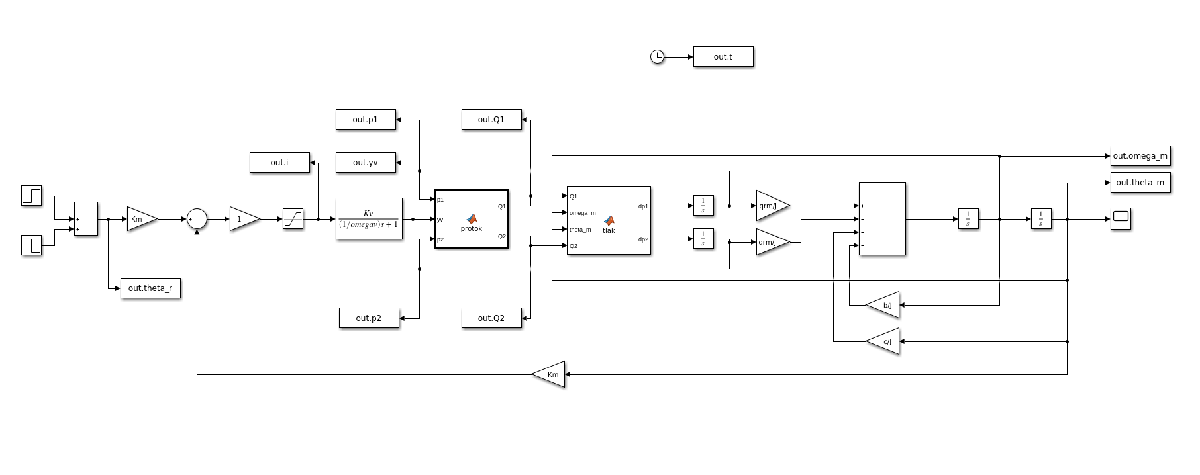
\includegraphics[width=\maxwidth{57.20020070245861em}]{image_1}
\end{flushleft}
\end{par}

\label{H_F4176A3E}
\matlabheadingtwo{Matlab funkcije u Simulinku}

\label{H_5282B22C}
\matlabheadingthree{Matlab funkcija protok}

\begin{par}
\begin{flushleft}
Funkcije protoka proporcionalnog ventila (2) i (3) su implementirane u Simulinku matlab funkcijom:
\end{flushleft}
\end{par}

\begin{verbatim}
function [Q1, Q2] = protok(p1, yv, p2)

ps = 100e5;
pa = 1e5;

if yv >= 0
    Q1 = yv * sqrt(abs(ps - p1)) * sign(ps - p1);
    Q2 = -yv * sqrt(abs(p2 - pa)) * sign(p2 - pa);
else
    Q1 = yv * sqrt(abs(p1 - pa)) * sign(p1 - pa);
    Q2 = -yv * sqrt(abs(ps - p2)) * sign(ps - p2);
end

end
\end{verbatim}

\vspace{1em}
\label{H_FDFA9491}
\matlabheadingthree{Matlab funkcija tlak}

\begin{par}
\begin{flushleft}
Funkcije ponašanja tlaka unutar dvije komore motora (8) i (9) su implementirane u Simulinku matlab funkcijom:
\end{flushleft}
\end{par}

\begin{verbatim}
function [dp1, dp2] = tlak(Q1, omega_m, theta_m, Q2)

qrm = 25.4e-6;
B = 1350e6;
V0 = 150e-6;

dp1 = (B/(V0 + qrm*theta_m) * (Q1 - qrm*omega_m));
dp2 = (B/(V0 - qrm*theta_m) * (Q2 + qrm*omega_m));

end
\end{verbatim}

\vspace{1em}
\label{H_FBEE3110}
\matlabheading{Simulacijski rezultati}

\label{H_D2F78E91}
\matlabheadingtwo{Pobuda i odziv}

\begin{matlabcode}
figure
subplot(2,1,1);
plot(out.t, out.theta_m, 'LineWidth', 2);
hold on
plot(out.t, out.theta_r, 'k--', 'LineWidth', 2);
grid on
xlabel('Vrijeme [s]');
ylabel('Kut zakreta \theta [rad]');
legend('Kut zakreta', 'Referenca');

subplot(2,1,2);
plot(out.t, out.omega_m, 'LineWidth', 2);
grid on
xlabel('Vrijeme [s]');
ylabel('Kutna brzina \omega [rad/s]');
\end{matlabcode}
\begin{center}
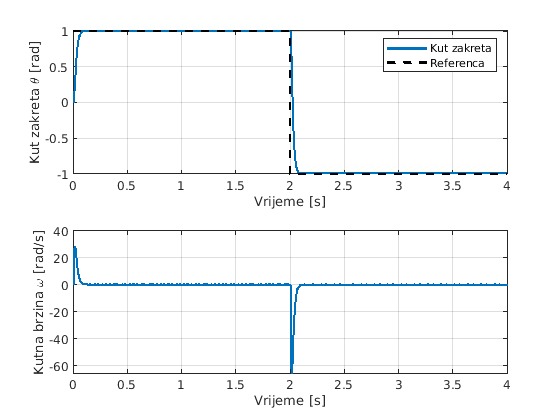
\includegraphics[width=\maxwidth{56.196688409433015em}]{figure_0.png}
\end{center}

\label{H_FD0E825B}
\begin{par}
\begin{flushleft}
Kut zakreta prati referencu aperiodski i vrijeme smirivanja je malo.
\end{flushleft}
\end{par}

\label{H_35364C80}

\vspace{1em}
\label{H_B10E4EC4}
\matlabheadingtwo{Pozicija proporcionalnog ventila}

\begin{matlabcode}
figure
subplot(2,1,1);
plot(out.t, out.i, 'LineWidth', 2);
grid on
xlabel('Vrijeme [s]');
ylabel('Struja i [A]');

subplot(2,1,2);
plot(out.t, out.yv, 'LineWidth', 2);
grid on
xlabel('Vrijeme [s]');
ylabel('Pozicija ventila yv [m]');
\end{matlabcode}
\begin{center}
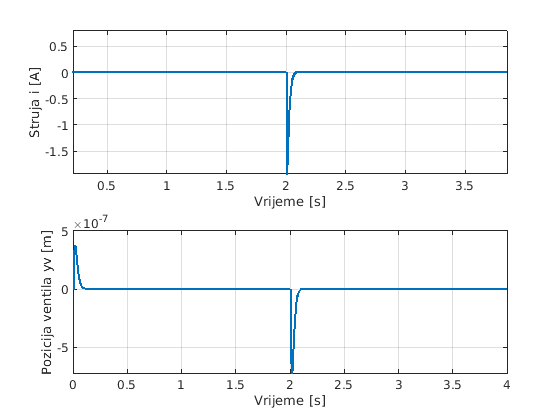
\includegraphics[width=\maxwidth{56.196688409433015em}]{figure_1.png}
\end{center}

\label{H_33C675A8}
\begin{par}
\begin{flushleft}
Grafovi pokazuju da je pozicija razvodnog klipa ventila proporcionaln struji. 
\end{flushleft}
\end{par}

\label{H_E57D2FC8}

\vspace{1em}
\label{H_8CBB40AD}
\matlabheadingtwo{Protok proporcionalnog ventila}

\begin{matlabcode}
figure
subplot(2,1,1);
plot(out.t, out.Q1, 'LineWidth', 2);
grid on
xlabel('Vrijeme [s]');
ylabel('Protok Q1 [m^3/s]');

subplot(2,1,2);
plot(out.t, out.Q2, 'LineWidth', 2);
grid on
xlabel('Vrijeme [s]');
ylabel('Protok Q2 [m^3/s]');
\end{matlabcode}
\begin{center}
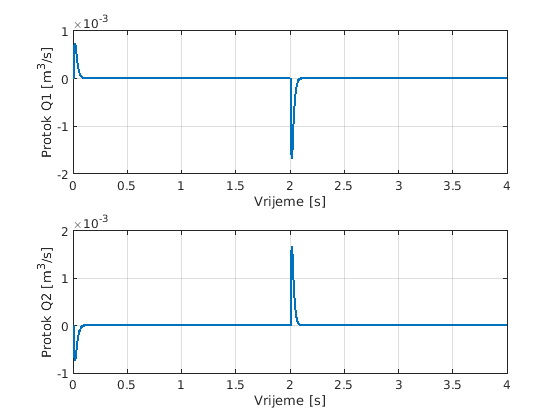
\includegraphics[width=\maxwidth{56.196688409433015em}]{figure_2.png}
\end{center}

\label{H_E7020DE1}

\vspace{1em}
\label{H_B43AD2CC}
\matlabheadingtwo{Tlakovi u komorama motora}

\begin{matlabcode}
figure
subplot(2,1,1);
plot(out.t, out.p1, 'LineWidth', 2);
grid on
xlabel('Vrijeme [s]');
ylabel('Tlak p1 [Pa]');

subplot(2,1,2);
plot(out.t, out.p2, 'LineWidth', 2);
grid on
xlabel('Vrijeme [s]');
ylabel('Tlak p2 [Pa]');
\end{matlabcode}
\begin{center}
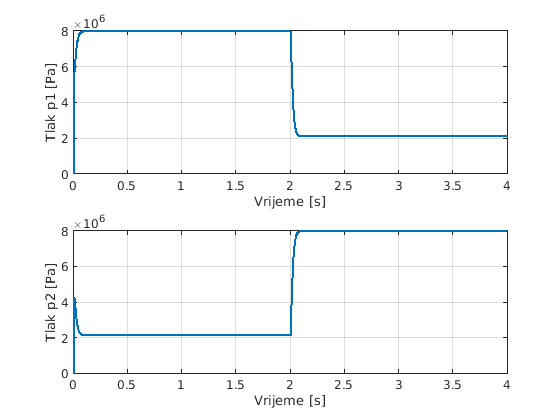
\includegraphics[width=\maxwidth{56.196688409433015em}]{figure_3.png}
\end{center}

\label{H_DD2B2F91}
\vspace{1em}

\label{H_FD72B4FF}
\matlabheading{Zaključak}


\vspace{1em}
\label{H_97AB6AE4}
\matlabheading{Prilog:}

\end{document}
